\chapter{Lenguaje de Actor Mínimo}

En este capítulo se explorará la gramática de un lenguaje que implementa los conceptos básicos vistos en la capitulo anterior, tales como comportamientos, creación de nuevos actores, creación de nuevas comunicaciones y otras construcciónes. El lenguaje \SAL fue desarrollado con intensiones pedagógicas y tiene una sintaxis heredada de Algol. 

Se utilizará la notación \textbf{Backus-Naur}\cite{McCracken:2003:BF:1074100.1074155} para describir la gramática. Adjunto a la notación se utilizá el símbolo \textbf{*} representa una o ninguna ocurrencias de un termino. 

\section{Expresiones}
Existen tres tipos primitivos, booleanos, enteros y dirección del buzón. Las operaciones posibles entre los booleanos \textbf{or}, \textbf{and}, \textbf{not}. Los enteros se pueden operar utilizando \textbf{+}, \textbf{-}, \textbf{*}, \textbf{/}. La dirección de un buzón es un identificador que es devuelto cuando se crea un nuevo actor, este tipo de primitivo no tiene ningún operador asociado.

La gramática de las expresiones booleanas es la siguiente:

\begin{grammar}

<bexp> ::= <bterm> `or' <bterm> | <bterm> `and' <bterm> 
  
<bterm> ::= <bool> | `not' <bterm> | `(' <bexp> `)' 

<bool> ::= `TRUE' | `FALSE'

\end{grammar}

La gramática de los enteros es la siguiente:

\begin{grammar}

<iexp> ::= <iterm> `*' <iterm> | <iterm> `/' <iterm>  
  \alt <iterm> `+' <iterm>  | <iterm> `-' <iterm>

<numero> ::= `1' | `2' | `3' | `4' | `5' | `6' | `7' | `8' | `9' | `0'

<iterm> ::= <numero> "*" | `-' <iterm> | `(' <iexp> `)'

\end{grammar}

La gramática de todas las expresiones:

\begin{grammar}
<exp> :: = <iexp> | <bexp> | <mexp> 
\end{grammar}

La gramática de $mexp$ es simplemente cualquier carácter entre la $A$ y la $Z$ tanto mayúscula como minúscula. 

\section{Definición de comandos}

% agregar referencia a la seccion de comandos
Los comandos son las acciones que permite a \SAL crear nuevos actores, enviar mensajes, definir un nuevo comportamiento. Estas describen en esencia lo que un actor puede hacer en un dentro de un comportamiento.

La gramática de los comandos en SAL es la siguiente:

\begin{grammar}
  <command> ::= `send' $exp_1, exp_2, \ldots\ , exp_n$ `to' <actor>  
  \alt `become' $B(exp_1, exp_2, ..., exp_n)$
  \alt `let' $mexp_1$ = `new' $B_1(exp_1, exp_2, ..., exp_{1n})$, \\
   \ldots\ \ $mexp_k$ = `new' $B_k(exp_1, exp_2, ..., exp_{kn})$   \\
  `in' <command> 
  \alt `if`<bexp> `then' <command> `else' <command> `end if'
\end{grammar}

\begin{description}
\item [send] Este comando permite enviar mensajes a otros actores, toma como parámetro una lista separada por coma de las expresiones a enviar, y el actor destino. El envío de mensajes es asincrónico. Cada expresión es evaluada antes utilizada como parámetro en \textit{acquaiantence-list}.
\item [become] Este comando especifica el siguiente comportamiento del actor que está procesando la comunicación recibida. Como en el caso anterior se evalúan las expresiones antes de utilizadas, y estas aparecerán como la listas de parámetros del comportamiento. 
\item[new] Este comando sirve para crear nuevos actores. El alcance de los
  identificadores de los nuevos actores creados está sujeto al cuerpo de \textbf{let}.
\item[condicional] Luego de evaluar la expresión booleana, si es verdadera
  ejecuta lo que esta a continuación de \textbf{then}, en caso contrario lo que está a
  continuación de \textbf{else}. Funciona como cualquier condicional.
\end{description}

La ejecución de los comandos ocurre cuando el actor recibe un mensaje, y todos
ellos ocurren concurrentemente, la composición no es secuencial.

\section{Definición de comportamientos}

La sintaxis de los comportamientos es la siguiente:

\begin{grammar}
<BDef> :== `def' <beh name> `(' <acquaiantence-list> `)' `[`'<input-list>`]' \\
\quad \quad <command>*  \\
\quad `end def'
  
<acquaiantence-list> :== <id> | ( <id> `,' <acquaiantence-list> ) *
  
<input-list> :== <id> | ( <id> `,' <input-list> ) *
\end{grammar}

El identificador \textit{beh name} hace referencia a un comportamiento y tiene alcance a todo el programa. 

Los identificadores \textit{acquaiantence-list} los recibe el momento de inicialización y tiene alcance en todo \textit{command}. 

Los identificadores \textit{input-list} son completados al momento de procesar una comunicación, y su alcance es todo \textit{command}. 

Podemos pensar que los comportamientos son una función que toma dos listas de parámetros en distintos momentos, uno cuando es inicializada o es invocada desde el cuerpo de un comando utilizando el comando $become$ y el otro conjunto de parámetros los recibe en e momento de procesar un mensaje.

Ambas listas, \textit{input-list} y \textit{acquaiantence-list} contienen todos los identificadores libres que están en \textit{command}. Existe un identificador especial \textit{self} que puede ser utilizado para hacer referencia al actor que está se definiendo. 

La ejecución de \textit{command} deberá contar a lo sumo con un solo comando \textit{become}, esta propiedad tiene que ser garantizado de manera estática, de no existir ningún comando \textit{become}, el actor asumirá un comportamiento de tipo \textit{bottom}, es es básicamente ignorar los mensajes que se le envíen.

\section{Ejemplos}

En esta sección mostraremos dos ejemplos de \SAL y algunas particularidades del lenguaje. Primero se presentará el código del ejemplo, a continuación una breve descripción linea por linea de la funcionalidad, y para terminar notas sobre su funcionamiento.

\subsection{Cálculo del factorial}

Está implementación del factorial está adaptada de \cite{Agha:1986:AMC:7929}. Depende de un actor \textit{main} que envía al actor $Factorial$ el valor a calcular, en el caso del ejemplo el valor $3$.

El actor factorial esta siempre disponible para procesar la siguiente comunicación, no bloquea con el calculo recursivo del factorial sino que lo delega en otros actores. Podemos notar, cuando factorial termina la ejecución el siguiente mensaje que procesa no necesariamente tiene que ver con la continuación de un calculo, sino que podría eventualmente procesar el pedido de otro cliente.

La palabra reservada \textit{self} hace referencia a este buzón, correspondiente al actor que está procesando la comunicación.

\begin{lstlisting}[language=sal, style=simple]
def Factorial()[val, customer]
  if val = 0 then
    send [1] to customer
  else
    let cont = new FactorialCont(val, customer)
       in send [val - 1, cont] to self
  end if 
  become Factorial()
end def

def FactorialCont(n, customer)[m] 
  send [n * m] to customer
end def

def Main() 
  let fact = new Factorial() 
    in send [3, self] to fact
end
\end{lstlisting}

\begin{description}

\item [Linea 1] $Factorial$ no recibe ningún parámetro en el momento de ser inicializado, pero si recibe dos parámetros cuando procesa una comunicación, la lista $[val, customer]$ un entero y una la dirección de un buzón respectivamente.
\item [Linea 2] Asigna como siguiente comportamiento a $Factorial()$, sin parámetros ya que $Factorial$ no recibe ningún parámetro a la inicialización.  
\item [Linea 4] Envía una lista con el valor $1$ al actor con buzón $customer$.
\item [Linea 6] Crea un actor de tipo $FactorialCont$. En este caso se utiliza $new$, ya que se está creando un nuevo buzón, y este se asigna a la variable $cont$. Cuando se asigna el nuevo comportamiento, este recibe los parámetros $val$ y $customer$.
\item [Linea 7] Envía un mensaje a la dirección del buzón propio utilizando la palabra reservada $self$, con la lista $val - 1$ y la dirección del buzón que se acaba de crear.
\item [Linea 11] $FactorialCont$ recibe dos valores cuando es instanciado: un entero $n$ y la dirección de un buzón $customer$. Cuando procesa un mensaje, en su \textit{acquaiantence-list} recibe un entero $m$.
\item [Linea 12] Envía la multiplicación $n*m$ como lista a la dirección del buzón $customer$ 
\item [Lineas 15-18] Inicializa el actor $Factorial$ y le envía a este la lista con los valores $3$ y la dirección del buzón actual. 

\end{description}

Concretamente, el actor ante un entero distinto de cero ejecuta dos acciones, crea un actor que espera un mensaje con un número y multiplicara este numero por \textbf{n} luego se enviará el resultado a el buzón de $customer$.

También, se envía un mensaje a si mismo para evaluar el factorial de \textbf{n - 1}, y como dirección de cliente utiliza la dirección del buzón del actor recientemente creado. Es decir el resultado de $fact(n - 1)$ se le pasará al actor recientemente creado que lo multiplicara por $n$.

Esto establece una red de actores que multiplicaran el valor indicado y enviaran el cálculo al siguiente actor en la red, y el último actor en la red se lo enviará a quien originalmente lo pidió.

En la figura \ref{fig:factorial} se puede ver que el actor $Factorial()$ recibe como comunicación la lista $[3,c]$, esto hace que ocurran dos cosas:

\begin{itemize}
\item Se cree un actor nuevo $FactorialCont$ con buzón $c1$, este recibe dos parámetros en la inicialización el valor $3$ y el buzón inicial que recibió como comunicación, es decir quien pidió originalmente la computación del factorial de $3$.

\item Se envíe a si mismo el mensaje $[2,c1]$, este inicia el calculo del factorial de $2$, es decir el cálculo de $fact(n-1)$, el paso recursivo.
\end{itemize}

Ahora $c1$ es quien pide el calculo del factorial de $2$. Esto se repite hasta que el valor a calcular es $0$.

Cuando el primer elemento de la comunicación es cero, hace que se le envíe al actor cuya dirección de buzón fue recién recibida, la lista con el valor uno. 

\begin{itemize}
\item $a$ le envía el valor $0$ a $c3$.
\item $c3$ multiplica $1*1$ y se lo envía a $c2$.
\item $c2$ multiplica $2*1$ y se lo envía a $c1$.
\item $c1$ multiplica $3*2$ y se lo envía a $c$.
\end{itemize}

Recordamos que $c$ había pedido el calculo del factorial $3$ en primer lugar.

\begin{figure}[H]
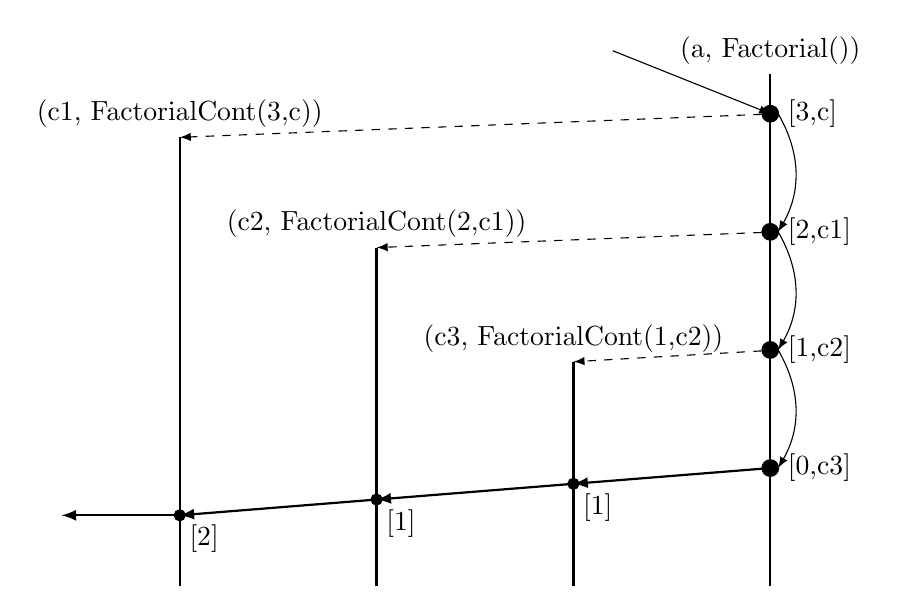
\begin{tikzpicture}

\draw[-latex] (6,7.3) to (8,6.5);

\draw[thick] (8,7) -- (8, 0.5);

\node[] (a1) at (8,7.3) {(a, Factorial())};

\node[align=center, right] (a1) at (8.1,6.5) {[3,c]};
\draw[fill] (8,6.5) circle (3pt);

\node[align=center, right] (a2) at (8.1,5) {[2,c1]};
\draw[fill] (8,5) circle (3pt);

\node[align=center, right] (a3) at (8.1,3.5) {[1,c2]};
\draw[fill] (8,3.5) circle (3pt);

\node[align=center, right] (a4) at (8.1,2) {[0,c3]};
\draw[fill] (8,2) circle (3pt);

\draw[-latex] (a1.west) to[bend left] (a2.west);
\draw[-latex] (a2.west) to[bend left] (a3.west);
\draw[-latex] (a3.west) to[bend left] (a4.west);

\node[] (d1) at (0.5,6.5) {(c1, FactorialCont(3,c))};
\draw[thick] (d1.south) -- (0.5, 0.5);

\node[] (c1) at (3,5.1) {(c2, FactorialCont(2,c1))};
\draw[thick] (c1.south) -- (3, 0.5);

\node[] (b1) at (5.5,3.65) {(c3, FactorialCont(1,c2))};
\draw[thick] (b1.south) -- (5.5, 0.5);

\draw[fill] (5.5,1.8) circle (2pt);
\node[align=center, right] (b2) at (5.5,1.5) {[1]};

\draw[fill] (3,1.6) circle (2pt);
\node[align=center, right] (c2) at (3,1.3) {[1]};

\draw[fill] (0.5,1.4) circle (2pt);
\node[align=center, right] (d2) at (0.5,1.1) {[2]};

\draw[-latex, thick] (8,2)  -- (5.5,1.8);
\draw[-latex, thick] (5.5,1.8) -- (3,1.6);
\draw[-latex, thick] (3,1.6) -- (0.5,1.4);
\draw[-latex, thick] (0.5,1.4) -- (-1,1.4);

\draw[-latex, black, dashed] (a1.west) -- (d1.south);
\draw[-latex, black, dashed] (a2.west) -- (c1.south);
\draw[-latex, black, dashed] (a3.west) -- (b1.south);
\end{tikzpicture}

\caption{El diagrama ilustra el cálculo del factorial de 3, todo el resultado es enviado al actor \textit{c}. Las lineas verticales indican el paso del tiempo, las de punto indican creación de actores y las otras flechas envío de mensaje. La lista superior indica  dirección del buzón, tipo de actor con los parámetros de inicialización.}

\label{fig:factorial}

\end{figure}
esta mas o menos 
\subsection{Una pila usando actores}

Otro ejemplo que podemos encontrar en \cite{Agha:1986:AMC:7929} es el de una pila, que está representada con una lista enlazada ordenada. Cada nodo de esta lista es un actor. 

Tiene dos operaciones básicas apilar ($push$), que coloca un nodo en la pila, y su operación inversa, sacar ($pop$), que remueve el último elemento agregado en la pila.

\begin{lstlisting}[language=sal, style=simple]
def node(content, link)[operation, customer, newcontent]
  if operation = pop then
    send content to customer
    become link
  enf if
  if operation = push then
    let P = new node(content, link)
      in become node(newcontent, P);
  end if
end def

def Main() 
  let stack = new node(10, Nil)
    in send [push, Nil, 20] to stack 
       send [push, Nil, 30] to stack
  end
end
\end{lstlisting}

\begin{description}

\item [Linea 1] $node$ está inicializado con dos parámetros, $content$ que es un entero, el valor que tiene que guardar el nodo y  $link$ es una dirección de buzón, es el siguiente actor en la pila. Recibe tres parámetros, $operation$ que es el tipo de operación a realizar,  $customer$ que se utiliza cuando la operación es $pop$, y $newcontent$ que se utiliza cuando la operación es $push$.
\item [Linea 3] La instrucción $become$, en este caso, hace que se reenvíen todos los mensajes a la dirección de buzón $link$. 
\item [Linea 4] Envía el contenido del nodo a la dirección de buzón $customer$
\item [Linea 7] Crea un nuevo actor con los parámetros de inicialización $content$ y $link$.
\item [Linea 8] Asigna el siguiente comportamiento, como $node$ con los parámetros $newcontent$ y la dirección de buzón del actor recién creado $P$. 
\item [Lineas 13-15] Crea una nueva pila con uno nodo con valor $10$, y envía dos operaciones $push$ con los valores $20$ y $30$.
\end{description}

El comportamiento $node$ funciona como una lista enlazada, donde en vez de tener direcciones de memoria tenemos direcciones de buzón. El primer parámetro es es el contenido a guardar $content$ y el segundo parámetro $link$ es el actor que está siguiente en la pila, el puntero al siguiente elemento.

Cuando $operation$ es de tipo $pop$, se envía el valor que contiene el nodo al buzón $customer$ y se reenvían todos los mensajes a $link$, todas las futuras operaciones $push$ y $pop$ las recibe este nodo, es decir que ahora es la ``cabeza'' de la pila. Esto guarda un parecido a mover un ``puntero''.

Cuando $operation$ es de tipo $push$, la pila crea un nuevo $node$ que sera el nodo que quedará siguiente en la red, se puede ver que esto ocurre en las lineas 7 y 8. Se copia en $P$ el nodo actual, y crea un nuevo nodo que es la nueva ``cabeza''.

Puede observarse en el ejemplo, que el primer nodo creado tiene como valor $Nil$, esto es simplemente una referencia nula. 